\chapter{Расчёт потоков на каждой из нескольких трещин гидроразрыва} \label{ch3}

Закачиваемый в скважину расход жидкости в общем случае перераспределяется между трещинами неодинаково вследствие разного качества перфораций на трещинах и других факторов.

В данной главе будет решена задача нахождения расхода $Q_i$ на каждой $i$-ой трещине и забойного давления $p_0$ при фиксированном расходе жидкости $Q_0$ на забое скважины.

\section{Постановка задачи}
\vspace*{-5mm}

На рис. \ref{fig:flow_distribution_scheme} представлена схема перераспределения потоков между тремя трещинами гидроразрыва пласта.
На этой схеме обозначены искомые $p_0$ (забойное давление), $Q_1$, $Q_2$, $Q_3$ (расходы жидкости на трещинах), а также величины, которые важно учитывать при расчёте потоков, так как их значения существенно влияют на конечный результат.

\begin{figure}[H] 
\center
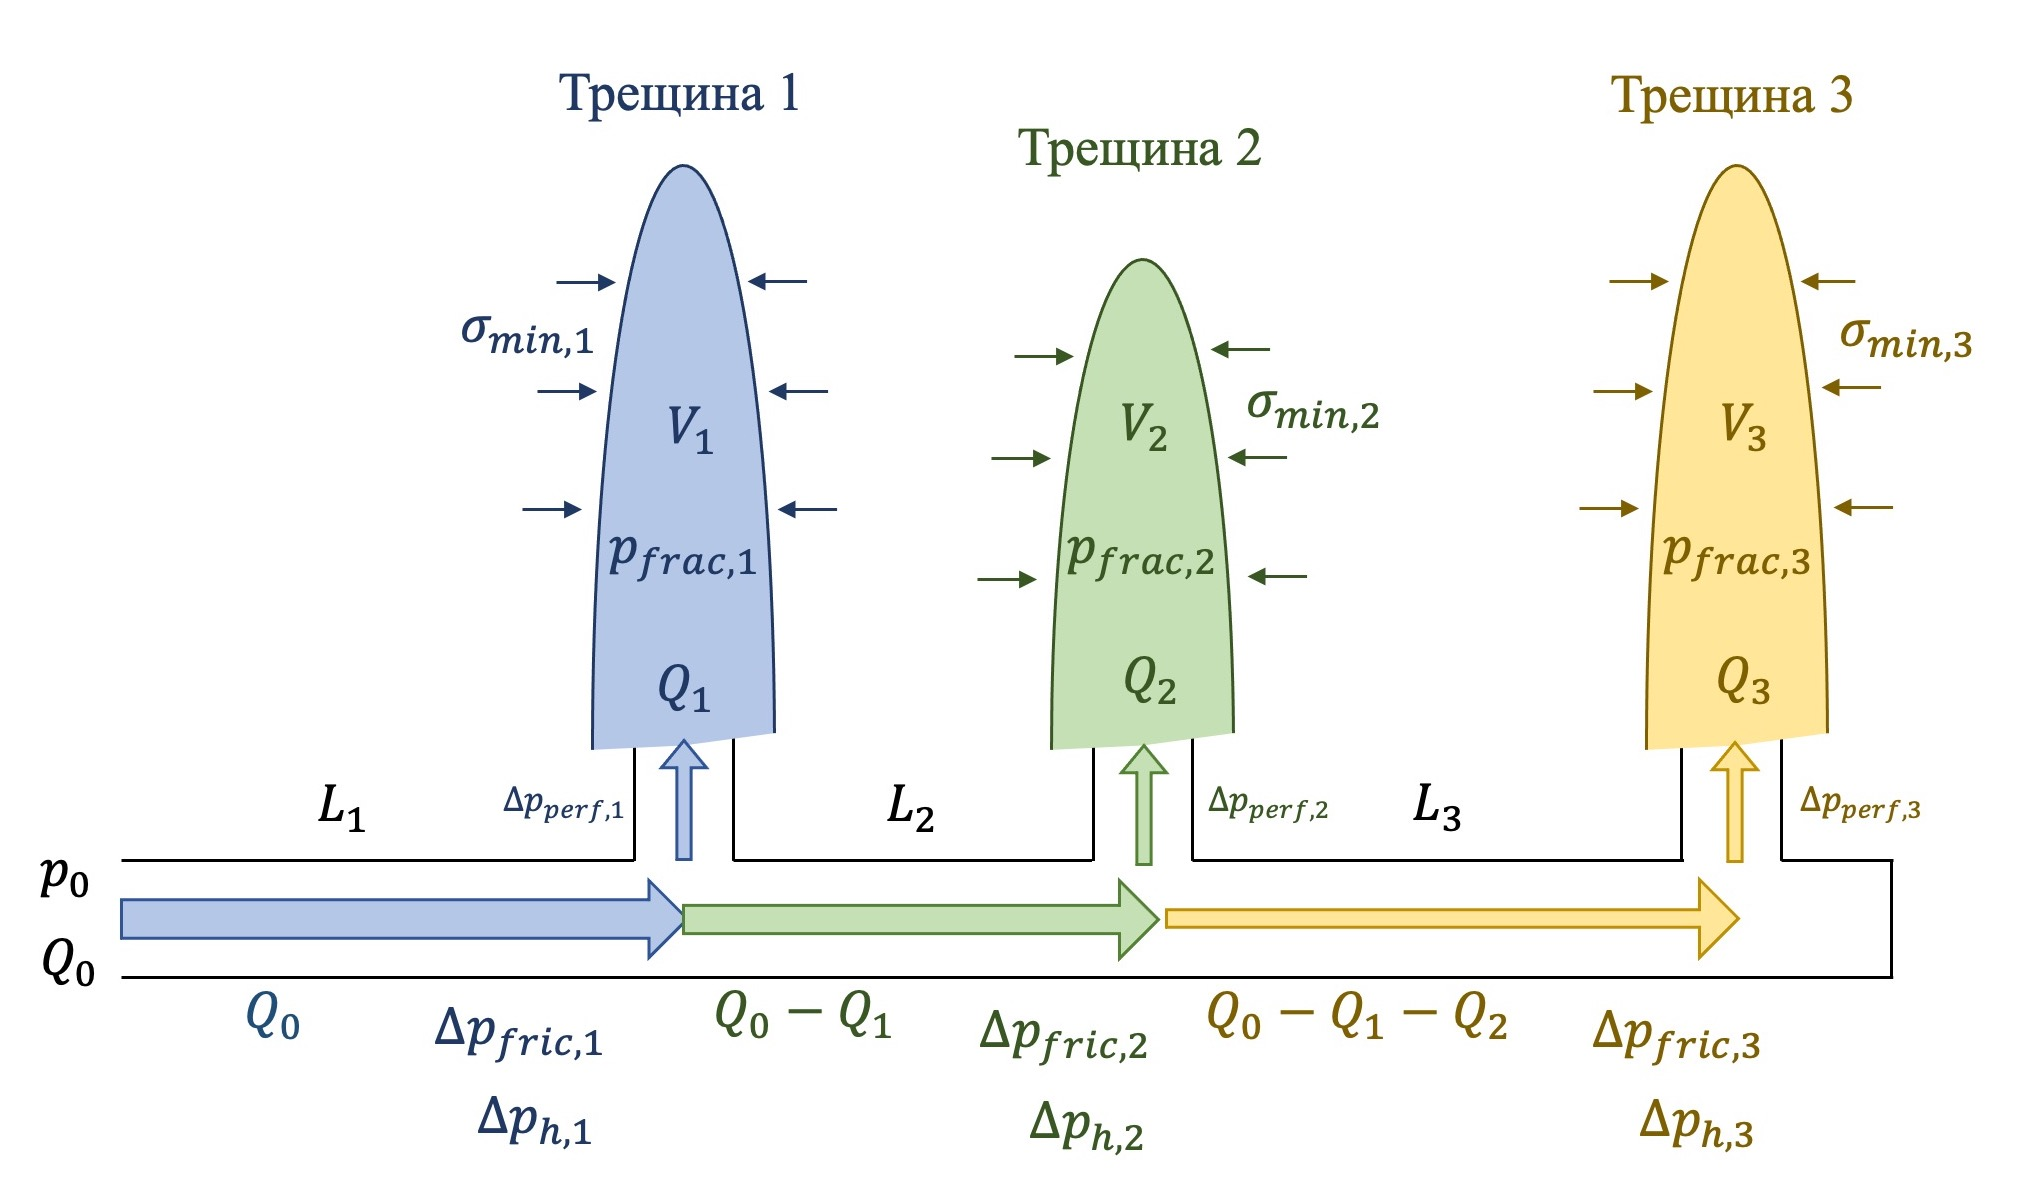
\includegraphics[width=\linewidth]{images/flow_distribution_scheme.jpg}
\caption{Схема перераспределения потоков между трещинами гидроразрыва} 
\label{fig:flow_distribution_scheme}  
\end{figure}

Согласно первому правилу Кирхгофа весь расход, который закачиваем в скважину, перераспределяется между трещинами:
\beq\label{3_1}
Q_0=\sum\limits_{i=1}^{N}Q_i,
\eeq
где $N$ -- количество трещин.

Согласно второму правилу Кирхгофа каждый из путей к каждой из трещин рассматривается независимо:
\beq\label{3_2}
p_0=\sigma_{\text{min},i}+p_{\text{net},i}+\Delta p_{\text{perf},i}-\sum_{j=1}^{i}{\Delta p_{h,j}}+\sum_{j=1}^{i}\Delta p_{\text{fric},j},
\eeq
где $\sigma_{\text{min},i}$ -- давление закрытия (минимальное напряжение в пласте) на $i$-ой трещине;\newline
$p_{\text{net},i}=p_{\text{frac},i}-\sigma_{\text{min},i}$ -- чистое давление на $i$-ой трещине (из модели трещины);\newline
$\Delta p_{\text{perf},i}$ -- падение давления вдоль перфорации $i$-ой трещины;\newline
$\Delta p_{\text{h},i}$ -- вклад гидростатического давления между $i$-ой и $(i-1)$-ой трещинами;\newline
$\Delta p_{\text{fric},i}$ -- падение давления на трение в трубе между $i$-ой и $(i-1)$-ой трещинами.

Объединяя уравнения \eqref{3_1} и \eqref{3_2}, получаем алгебраическую систему уравнений относительно $p_0$ и $Q_i$ (где $i=\overline{1, N}$).
Чтобы решить эту систему из $N+1$ уравнений с $N+1$ неизвестной, необходимо получить замыкающие соотношения на $p_{\text{net},i}$, $\Delta p_{\text{perf},i}$ и $\Delta p_{\text{fric},j}$.
Другими словами, необходимо получить зависимости этих величин от искомых величин $p_0$, $Q_i$ и других параметров, значения которых можно найти непосредственным измерением или задать при проектировании скважины.

\section{Замыкающие соотношения}
\vspace*{-5mm}

\textbf{Выражение для чистого давления в трещине автоГРП}

В работе \cite{kabanova_shel} получена формула для чистого давления трещины Перкинса-Керна-Нордгрена (модели PKN):
\beq\label{1_3}
p_{\text{net},i}=\sqrt{\frac{8K_{Ic,i}^2}{\pi h_{f,i}}},
\eeq
где $K_{Ic,i}$ -- трещиностойкость породы вблизи $i$-ой трещины,\newline
$h_{f,i}$ -- высота $i$-ой трещины (в случае PKN модели равна мощности продуктивной зоны).
\\

\textbf{Выражение для падения давления на перфорациях}

Эмпирическая формула для падения давления на перфорациях \cite{crump,cramer,gongbo} выглядит следующим образом:
\beq\label{1_4}
\Delta p_{\text{perf},i}=\frac{8\rho_s}{\pi^2 C_{d,i}^2 n_{p,i}^2 d_{p,i}^4}Q_i\left|Q_i\right|,
\eeq
где $\rho_s$ -- средняя плотность смеси;\newline
$n_{p,i}, d_{p,i}$ -- количество и диаметр перфораций;\newline\\
$C_{d,i}=\dfrac{\text{min}(d_{jet})}{d_p}$ -- безразмерный коэффициент эрозии (в случае отсутствия твёрдых частичек в потоке $C_{d,i}\in\left[0.5,0.6\right]$, а с твёрдыми частичками в потоке $C_{d,j}\in\left[0.6,0.95\right]$  из-за эрозии перфорации).
\\

\textbf{Выражение для падения давления на трение в трубе}

Для того, чтобы получить формулу для падения давления на трение в трубе, запишем уравнение Навье-Стокса и усредним его по площади сечения трубы:
\beq
0=-\frac{dp(x)}{dx}+\frac{1}{r}\frac{d}{dr}\left(r\tau_{rx}\right)+\rho g \sin{\theta}\,\,\,\bigg|\,\,\,\,\,\frac{1}{\pi R^2}\int\limits_{S}\left(\cdot\right)dS,
\eeq
где $dp(x)/dx$ -- падение давления вдоль скважины;
$\tau_{rx}$ -- напряжение сдвига;
$\rho$ -- плотность жидкости;
$\theta$ -- угол между скважиной (нормалью к сечению трубы) и поверхностью земли.

После усреднения получаем следующее уравнение (среднее $\bar{p}$ на самом деле можно заменить на просто $p$, так как давление выравнивается вдоль сечения -- это можно доказать в предположениях течения тонкого слоя):
\beq\label{Navie_average}
\frac{d\bar{p}}{dx}=-\frac{2\tau_w}{R}+\bar{\rho}g\sin{\theta},
\eeq
где $\tau_w=-\tau_{rx}|_{r=R}$ -- напряжение сдвига (трения) на стенке трубы.
Это напряжение сдвига (трения) можно измерить при ламинарном течении, а также в случае турбулентного течения (например, для известного перепада давления найти $\tau_w$ из \eqref{Navie_average} -- то есть решить обратную задачу).

Введём коэффициент трения Фаннинга
\beq
f_s=\frac{\tau_w}{\rho u_m^2/2},
\eeq
где $u_m$ -- средняя скорость потока в рассматриваемом сечении трубы.

Тогда уравнение \eqref{Navie_average} примет следующий вид:
\beq
\frac{dp}{dx}=\underbrace{-\frac{\rho u_m^2}{R}f_s}_{\text{на трение}}\,+\underbrace{\rho g\sin{\theta}}_{\substack{\text{вклад}\\\text{гидро-}\\\text{статического}\\\text{давления}}}
\eeq
Получили уравнение баланса сил: сила давления и сила тяжести уравновешиваются силой трения жидкости о стенки трубы.

Таким образом, падение давления на трение на каждом интервале рассчитывается по следующей формуле:
\beq\label{3_5}
\Delta p_{\text{fric},i}=\int\limits_{x_{i-1}}^{x_i}{f_s\frac{\rho u_{m,i}^2}{R_i}}=\int\limits_{x_{i-1}}^{x_i}{\frac{\rho(c(t,s))\cdot f(Re)\cdot \left(Q_0-\sum\limits_{j=1}^{i-1}{Q_j}\right)^{\!2}}{R_i(s)S_i^2(s)}}ds,
\eeq
где $f_s=\dfrac{\tau_w}{\rho u_{m,i}^2/2}$ -- коэффициент трения Фаннинга;\newline\\
$\rho(c(t,s))$ -- плотность смеси, которая зависит от динамически меняющейся концентрации проппанта;\newline\\
$u_{m,i}=\dfrac{Q_0-\sum\limits_{j=1}^{i-1}{Q_j}}{S_i}$ -- средняя скорость в рассматриваемом сечении участка трубы;\newline
$S_i$ -- площадь сечения рассматриваемого участка трубы;\newline
$R_i$ -- радиус рассматриваемого участка трубы;\newline
$Re$ -- число Рейнольдса.

Для ламинарного режима течения ньютоновской жидкости:
\beq
u_x=2u_m\left(1-\frac{r^2}{R^2}\right)\,\,\,\text{ и }\,\,\,\tau_w=-\mu_s\frac{\partial u_x}{\partial r}\bigg|_{r=R}=\frac{4\mu_s u_m}{R},
\eeq
где $\mu_s$ -- вязкость закачиваемой в скважину жидкости.\newline
Тогда коэффициент трения Фаннинга для ламинарного режима течения запишется в следующем виде:
\beq
f_s=\frac{\tau_w}{\rho u_m^2/2}=\frac{8\mu_s}{\rho Ru_m}=\frac{16}{Re},
\eeq
где $Re=\dfrac{\rho u_m\left(2R\right)}{\mu_s}$ -- число Рейнольдса \cite{reynolds}.

В трещины автоГРП закачивается вода без дополнительных веществ, поэтому плотность закачиваемой жидкости постоянна по всей длине скважины и равна плотности воды.

Таким образом, в случае ламинарного режима течения однородной ньютоновской жидкости (например, воды) формула для падения давления на трение в трубе \eqref{3_5} упрощается и запишется в следующем виде:
\beq
\Delta p_{\text{fric}, i}=\int\limits_{x_{i-1}}^{x_i}{\frac{8\mu\left(Q_0-\sum\limits_{j=1}^{i-1}{Q_j}\right)}{R_i^2(s)S_i(s)}}ds,
\eeq
где $\mu$ -- вязкость воды.
\\

\textbf{Выражение для изменения гидростатического давления}

В общем случае изменение гидростатического давления на каждом интервале рассчитывается по следующей формуле:
\beq
\Delta p_{h,i}(t,x)=\int\limits_{x_{i-1}}^{x_i}{\rho(c(t,s))\cdot g\cdot \sin{\theta(s)}ds},
\eeq
где
$x_i$ -- измеренная глубина (MD) $i$-ого порта ГРП;\newline
$\rho(c(t,s))$ -- плотность закачиваемой в скважину смеси, которая зависит от меняющейся с координатой и временем концентрации проппанта;\newline
$g$ -- ускорение свободного падения;
$\theta(s)$ -- угол между скважиной (нормалью к сечению трубы) и поверхностью земли в текущем заданном сечении трубы.

В данной работе исследуется поведение трещин, которые распространяются от одной горизонтальной скважины в одном пласте, залегающем на фиксированной глубине, поэтому изменения гидростатического давления между портами ГРП нет:
\beq
\Delta p_{h,i}=0.
\eeq

\textbf{Замкнутая постановка задачи}

С учётом полученных замыкающих соотношений постановка задачи о расчёте потоков между трещинами автоГРП запишется в следующем виде:

\beq\label{flows_statement}
\begin{cases}
	\displaystyle Q_0=\sum\limits_{i=1}^{N}Q_i,\\
	\displaystyle p_0=\sigma_{\text{min},i}+p_{\text{net},i}+\Delta p_{\text{perf},i}-\sum_{j=1}^{i}{\Delta p_{h,j}}+\sum_{j=1}^{i}\Delta p_{\text{fric},j},\\[10pt]
	\displaystyle p_{\text{net},i}=\sqrt{\dfrac{8K_{Ic,i}^2}{\pi h_{f,i}}},\\[15pt]
	\displaystyle \Delta p_{\text{perf},i}=\dfrac{8\rho_s}{\pi^2 C_{d,i}^2 n_{p,i}^2 d_{p,i}^4}Q_i\left|Q_i\right|,\\[15pt]
	\displaystyle \Delta p_{\text{fric}, j}=\int\limits_{x_{j-1}}^{x_j}{\dfrac{8\mu\left(Q_0-\sum\limits_{k=1}^{j-1}{Q_k}\right)}{R_j^2(s)S_j(s)}}ds,\\
	\displaystyle \Delta p_{h,j}=0.
\end{cases}
\eeq

Подстановка последних четырёх равенств \eqref{flows_statement} в первые два равенства даёт замкнутую систему нелинейных алгебраических уравнений с неизвестными $p_0$ и $Q_i$ ($i=\overline{1,N}$), которая может быть решена численно, например, с помощью метода Ньютона.

\section{Описание численного алгоритма решения}
\vspace*{-5mm}

Используя замкнутую постановку задачи \eqref{flows_statement}, введём вектор неизвестных $Q^{T}=\left[Q_1,Q_2,...,Q_N,p_0\right]$ и вектор невязок $F^{T}=\left[F_1,F_2,...,F_N, F_{N+1}\right]$, где
\beq
F_i=
\begin{cases}
\displaystyle \sigma_{\text{min},i}+p_{\text{net},i}+\Delta p_{\text{perf},i}-\sum\limits_{j=1}^{i}{\Delta p_{h,j}}+\sum\limits_{j=1}^{i}{\Delta p_{\text{fric},j}}-p_0\\[-2pt]\,\,\,\,\,\,\,\,\,\,\,\,\,\,\,\,\,\,\,\,\,\,\,\,\,\,\,\,\,\,\,\,\,\,\,\,\,\,\,\,\,\,\,\,\,\,\,\left(\text{при }i\leqslant N\right)\\[15pt]
\displaystyle Q_0-\sum\limits_{j=1}^{N}{Q_j}\left(\text{при }i=N+1\right)
\end{cases}
\eeq

Ставится задача минимизации вектора невязок.
В качестве начального приближения считается, что закачиваемый в скважину расход жидкости перераспределяется между трещинами одинаково $Q_i=Q_0/N$ (где $i=\overline{1,N}$), а забойное давление принимается равным давлению закрытия (смыкания) трещин $p_0=\sigma_{\text{min}}$.

Далее составляется матрица Якоби
\beq
J=
\begin{bmatrix}
	\dfrac{\partial F_1}{\partial Q_1} & \dots & \dfrac{\partial F_1}{\partial Q_N} & \dfrac{\partial F_1}{\partial p_0} \\
	\vdots & \ddots & \vdots & \vdots \\
	\dfrac{\partial F_{N+1}}{\partial Q_1} & \dots & \dfrac{\partial F_{N+1}}{\partial Q_N} & \dfrac{\partial F_{N+1}}{\partial p_0} \\
\end{bmatrix}
\eeq
и итеративно с помощью метода Ньютона ищется вектор неизвестных $Q^{T}$:
\beq
\overline{Q}^{k+1}=\overline{Q}^k-J^{-1}\overline{F}^k
\eeq
В качестве условия остановки выбрано следующее условие на разницу между соседними приближениями к решению:
\beq
\left|\overline{Q}^{k+1}-\overline{Q}^k\right|^2\leqslant10^{-4}.
\eeq

Реализация описанного численного алгоритма решения на языке программирования Python представлена в приложении 1.

\section{Результаты}
\vspace*{-5mm}

Значения входных параметров, выбранные перед запуском алгоритма представлены в таблице \ref{tab:input-parameters-for-flow-splitting}.

\newcolumntype{L}[1]{>{\raggedright\arraybackslash}m{#1}}
\newcolumntype{C}[1]{>{\centering\arraybackslash}p{#1}}
\noindent % for correct centering
\begingroup
\small %выставляем шрифт в 12bp
\begin{longtable}[l]{|C{8cm}|C{8cm}|}
	\caption{Значения входных параметров алгоритма расчёта потоков}%
	\label{tab:input-parameters-for-flow-splitting}% label всегда желательно идти после caption
	\\
	\hline
	\multicolumn{1}{|c|}{\textbf{Параметр}}&\multicolumn{1}{|c|}{\textbf{Значение}}\\ \hline
	\endfirsthead%
	\captionsetup{format=tablenocaption,labelformat=continued} % до caption!
	\caption[]{}\\ % печать слов о продолжении таблицы
	\hline
	\multicolumn{1}{|c|}{\textbf{Параметр}}&\multicolumn{1}{|c|}{\textbf{Значение}}\\ \hline
	\endhead
	\hline
	\endfoot
	\hline
	\endlastfoot
	Расход на забое $Q_0$&800 м$^3$/сут\\ \hline
	Вязкость закачиваемой жидкости (воды) $\mu$ & $10^{-3}$ Па$\cdot$с\\ \hline
	Плотность закачиваемой жидкости (воды) $\rho$ & 1000 кг/м$^3$\\ \hline
	Проницаемость пласта $k_e$ & 1 мД\\ \hline
	Пористость пласта $\varphi_e$ & 0.2\\ \hline
	Общая сжимаемость $c_t$ & $2.2\cdot 10^{-9}$ Па$^{-1}$\\ \hline
	Пластовое давление $p_e$ & 25 МПа\\ \hline
	Модуль плоской деформации породы $E'$ & $10^4$ МПа\\ \hline
	Мощность пласта $H$ & 15 м\\ \hline
	Количество перфораций $n_p$ & 32\\ \hline
	Диаметр перфораций $d_p$ & 0.02 м\\ \hline
	Безразмерный коэффициент эрозии $C_d$ & 0.5\\ \hline
	Радиус участков трубы $R$ & 0.08 м\\ \hline
	Длина участков трубы $L$ & 100 м\\ \hline
	Давление смыкания $\sigma_{\text{min}}$ & 40 МПа\\ \hline
	Трещиностойкость породы $K_{Ic}$ & $10^6$ Па$\cdot$м$^{1/2}$\\ \hline
	Количество трещин & 4\\ \hline
\end{longtable}
\normalsize% возвращаем шрифт к нормальному
\endgroup

На рис \ref{fig:flows_distribution_between_fractures_1} показан итеративный процесс поиска расходов жидкости на каждой из четырёх трещин автоГРП.

\begin{figure}[H] 
\center
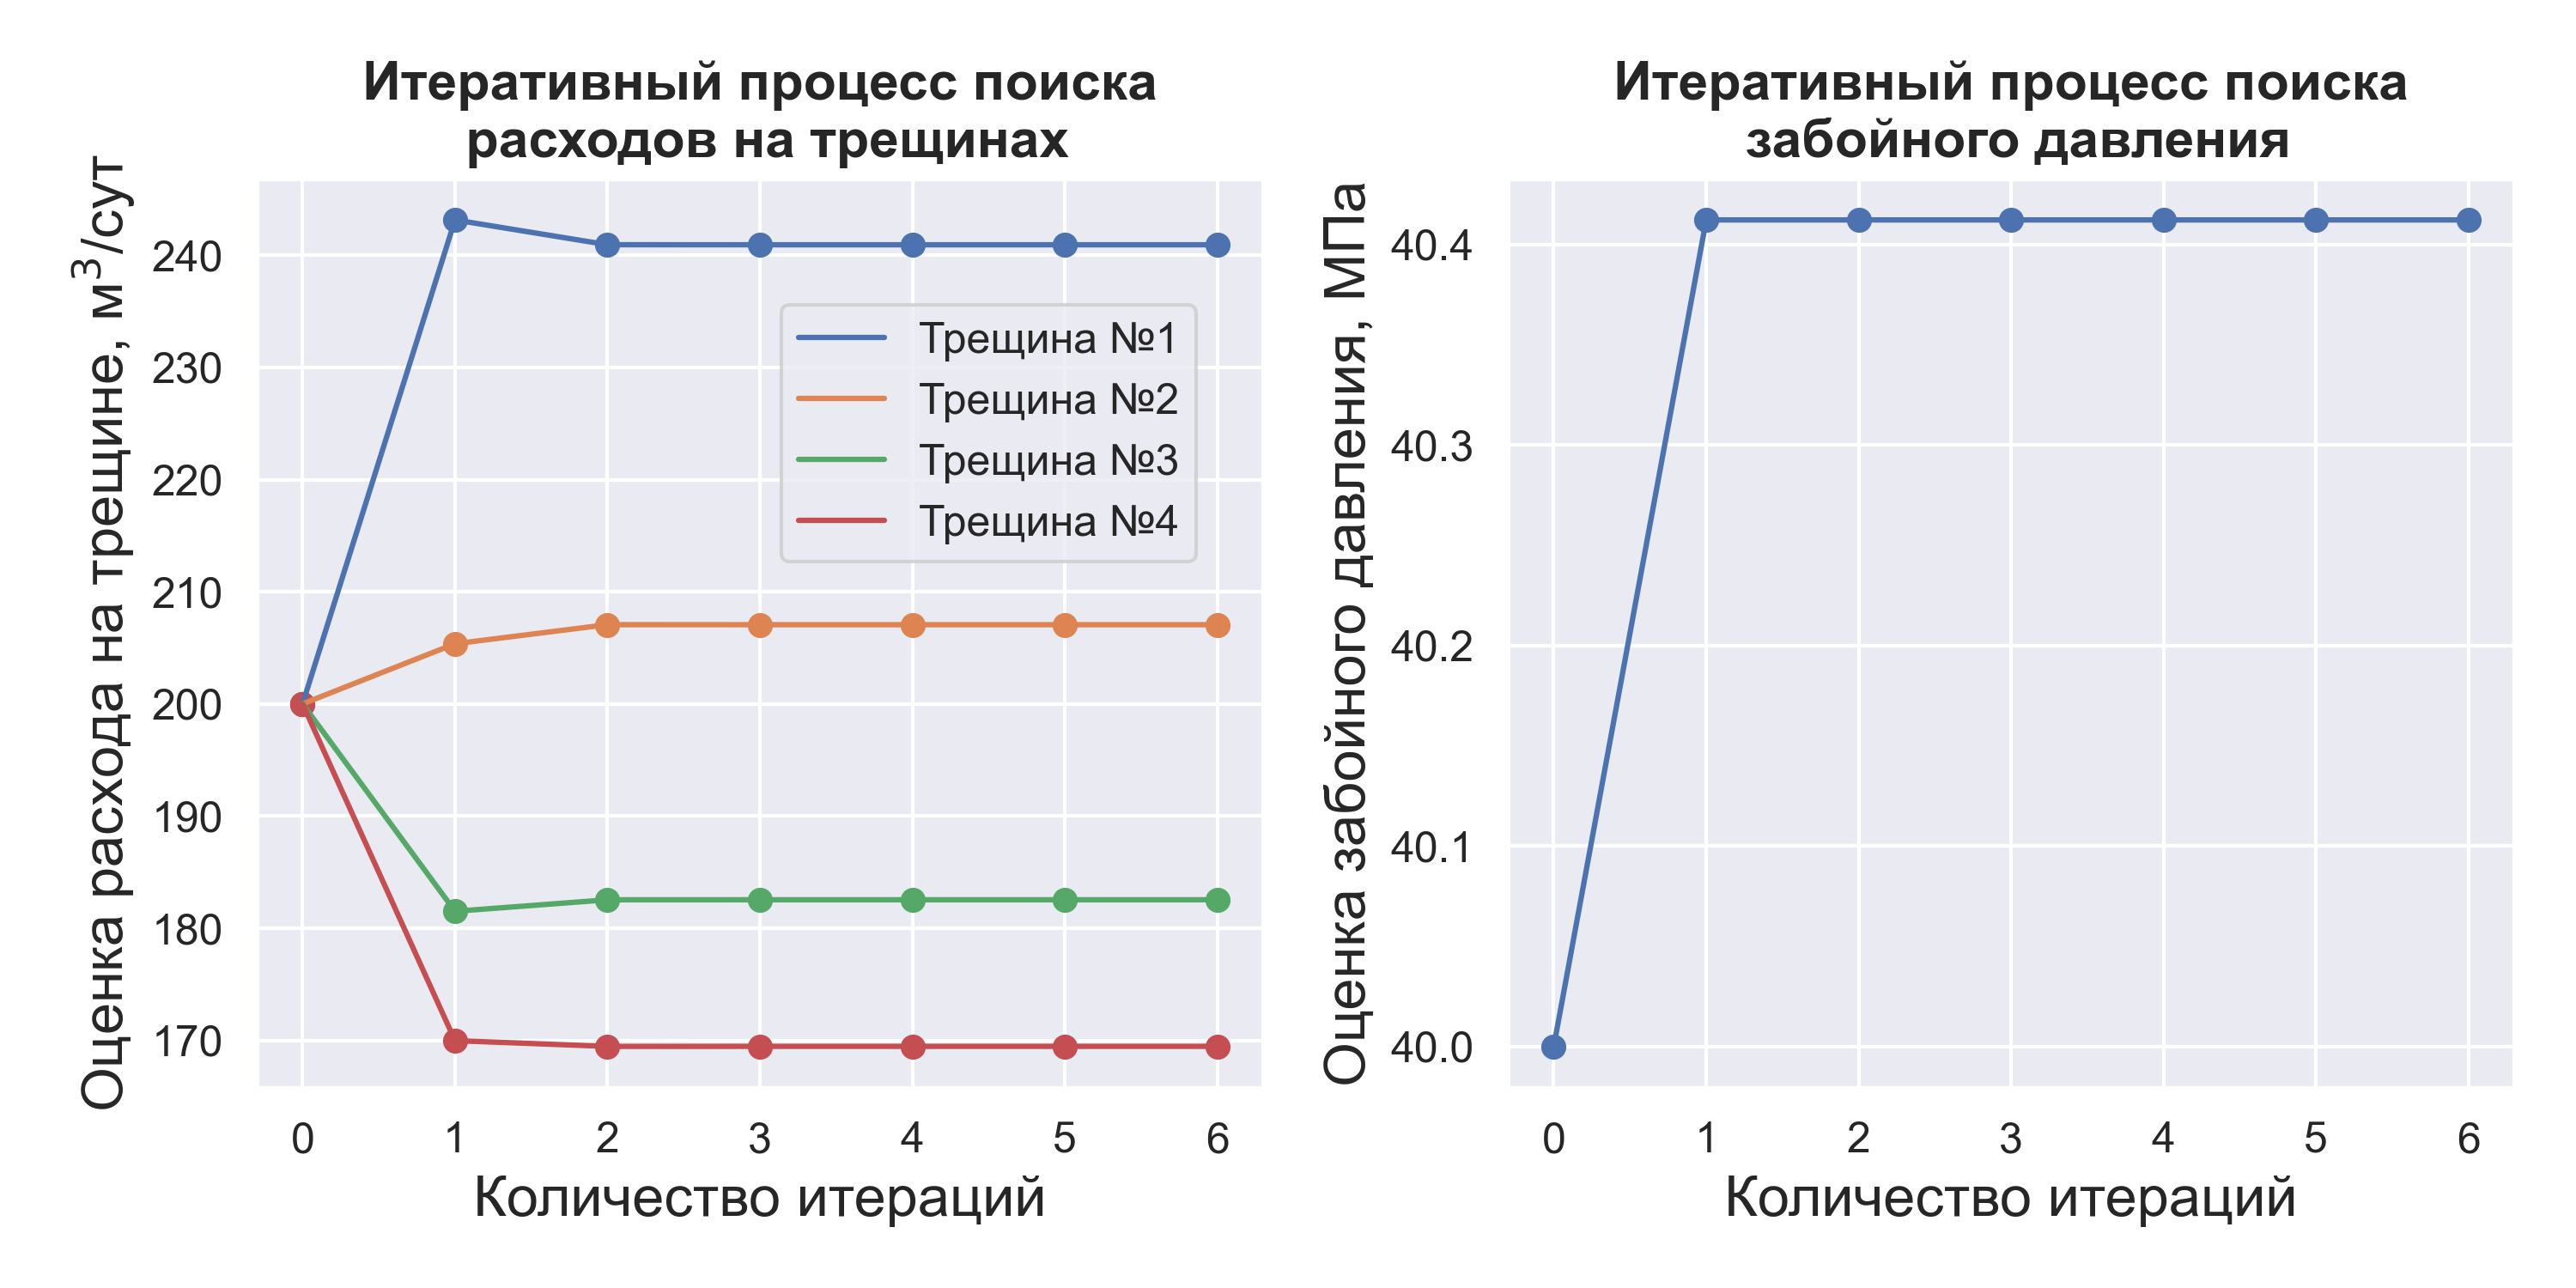
\includegraphics[width=\linewidth]{images/flows_distribution_between_fractures_1.jpg}
\caption{Итеративный процесс поиска расходов на трещинах и забойного давления (входные параметры алгоритма представлены в таблице \ref{tab:input-parameters-for-flow-splitting})}
\label{fig:flows_distribution_between_fractures_1}  
\end{figure}

Видим, что потоки распределились по трещинам неодинаково вследствие имеющихся потерь давления на трения в трубе (падение давления на трение при движении жидкости к первой трещине меньше, чем падение давления на трение при движении жидкости по трубе к последней трещине).

Далее проведён расчёт потоков на каждой из четырёх трещин в случае уменьшенного диаметра перфораций на второй трещине (диаметр уменьшен с $0.02$ м до $0.005$ м).
Результаты представлены на рис. \ref{fig:flows_distribution_between_fractures_2}.

\begin{figure}[H] 
\center
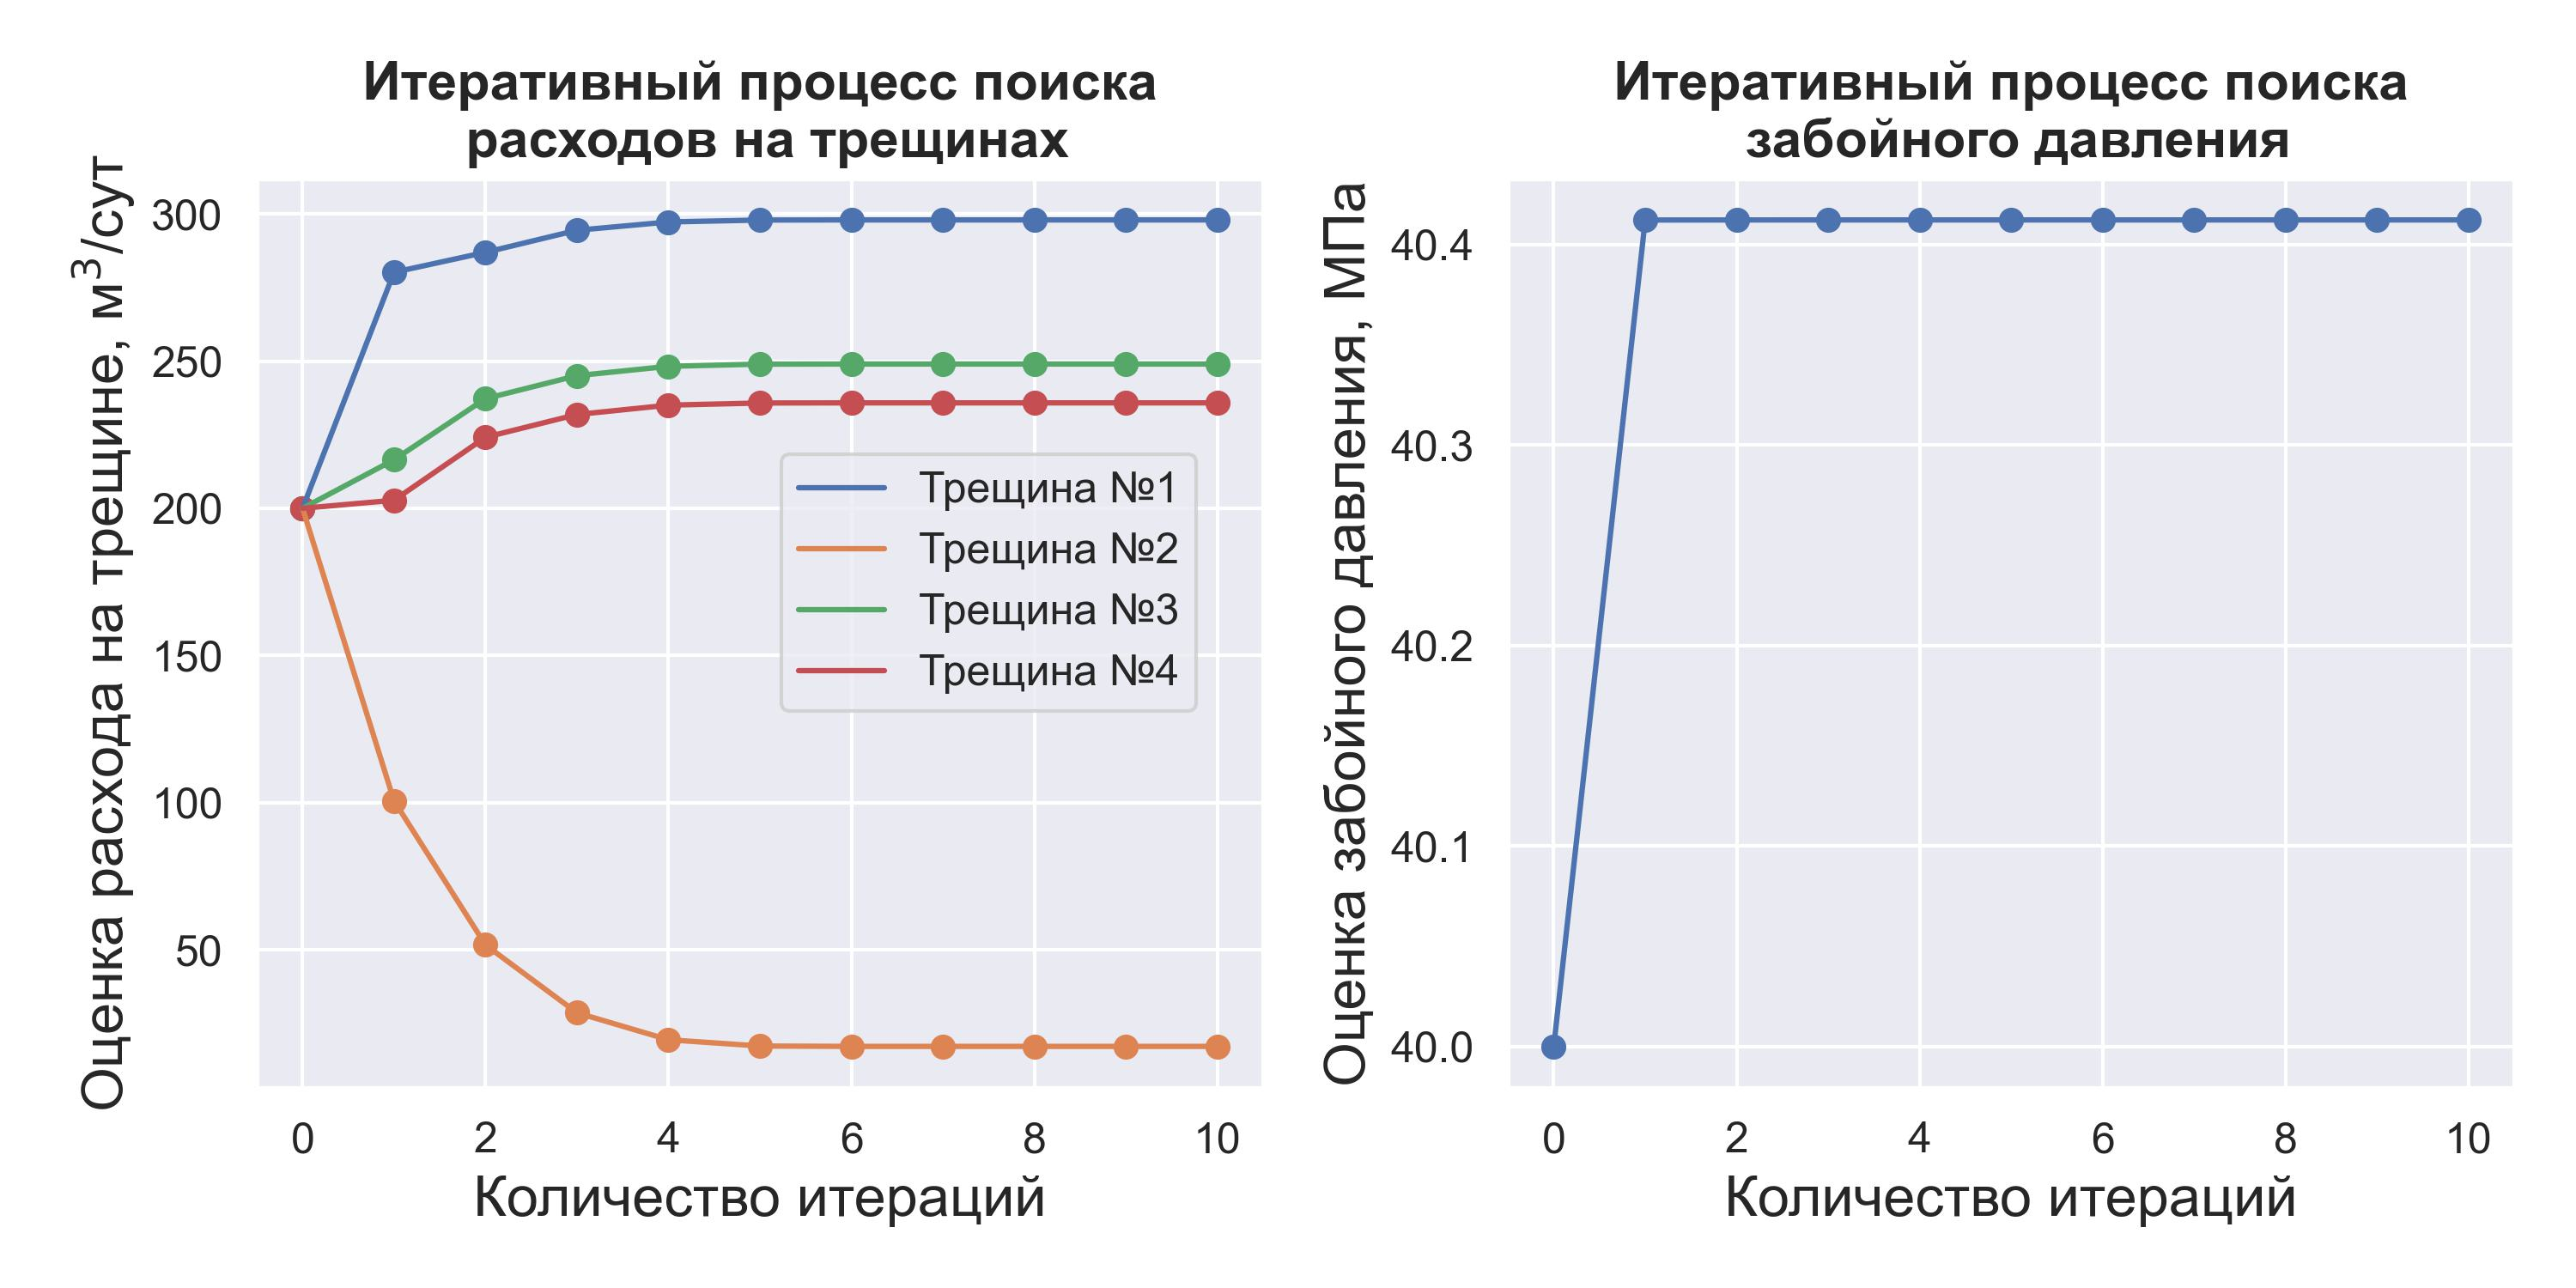
\includegraphics[width=\linewidth]{images/flows_distribution_between_fractures_2.jpg}
\caption{Итеративный процесс поиска расходов на трещинах и забойного давления (по сравнению с предыдущим расчётом уменьшен диаметр перфораций $d_{p,2}=0.005$ м на второй трещине)}
\label{fig:flows_distribution_between_fractures_2}  
\end{figure}

Видим, что уменьшение диаметра перфораций на одной из трещин существенно сократило расход жидкости на этой трещине и при этом возросли расходы жидкости на соседних трещинах.

Итак, в данной главе реализован алгоритм расчёта потоков на каждой из нескольких трещин автоГРП.
В следующей главе этот алгоритм будет использован для моделирования одновременного роста нескольких трещин автоГРП в длину.
